\documentclass{standalone}
\usepackage{standalone}

\begin{document}
\subsection{Converting to Gray-Scale}
From the 24-bit color image, we split the $R$, $G$, $B$ components of each pixels $(i, j)$. Then, 8-bit gray-value is calculated by using the Equation \ref{eq:GrayEquation}. A sample result is shown in Figure \ref{fig:GraySample}.

\begin{equation}\label{eq:GrayEquation}
gray(i, j) = 0.11 * B(i, j) + 0.30 * G(i, j) + 0.59 * R(i, j)
\end{equation}

\begin{figure}
	\centering
	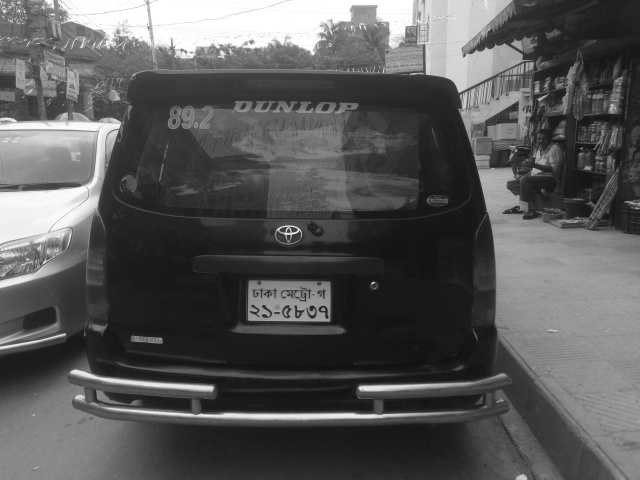
\includegraphics[width=.8\linewidth]{./img/sample/stage1.jpg}
	\caption{A sample gray-scale image} 
	 \label{fig:GraySample}
\end{figure}

\end{document}